\section{Simulation Analysis}
\label{sec:simulation}

In this section we wrote a \textit{Ngspice} script to simulate the Band-Pass 
filter circuit described in \ref{fig:circuit}, using the OP-AMP model provided in the .net script.
Finally we measured the output voltage gain in the passband, the central frequency, the maximum gain, and the input and output impedances.

To begin with, we started with a time analysis of the circuit, followed by its frequency analysis. In order to calculate the gain in the central frequency, we obtained the maximum of the output gain, in dB. 
The central frequency was the correponding frequency. To calculate the input impedance, we used Ohm's law in the input source, whereas for the output impedance, a secondary .net file was created with a test source at the output. 

The cost of the circuit designed is (custo).


\section{Side-By-Side Comparison}
\label{sec:side}

In this section, we show the results obtained in both the theoritcal and simulation analysis side-by-side. More specifically, we show the comparison between the gain graphs, the phase graphs and the impendances, maximum gain and central frequency values.

\begin{figure*}[h]
    \centering
    \begin{subfigure}{0.5\textwidth}
      \includegraphics[width=\linewidth, clip]{gain.eps}
    \end{subfigure}
    \begin{subfigure}{0.4\textwidth}
      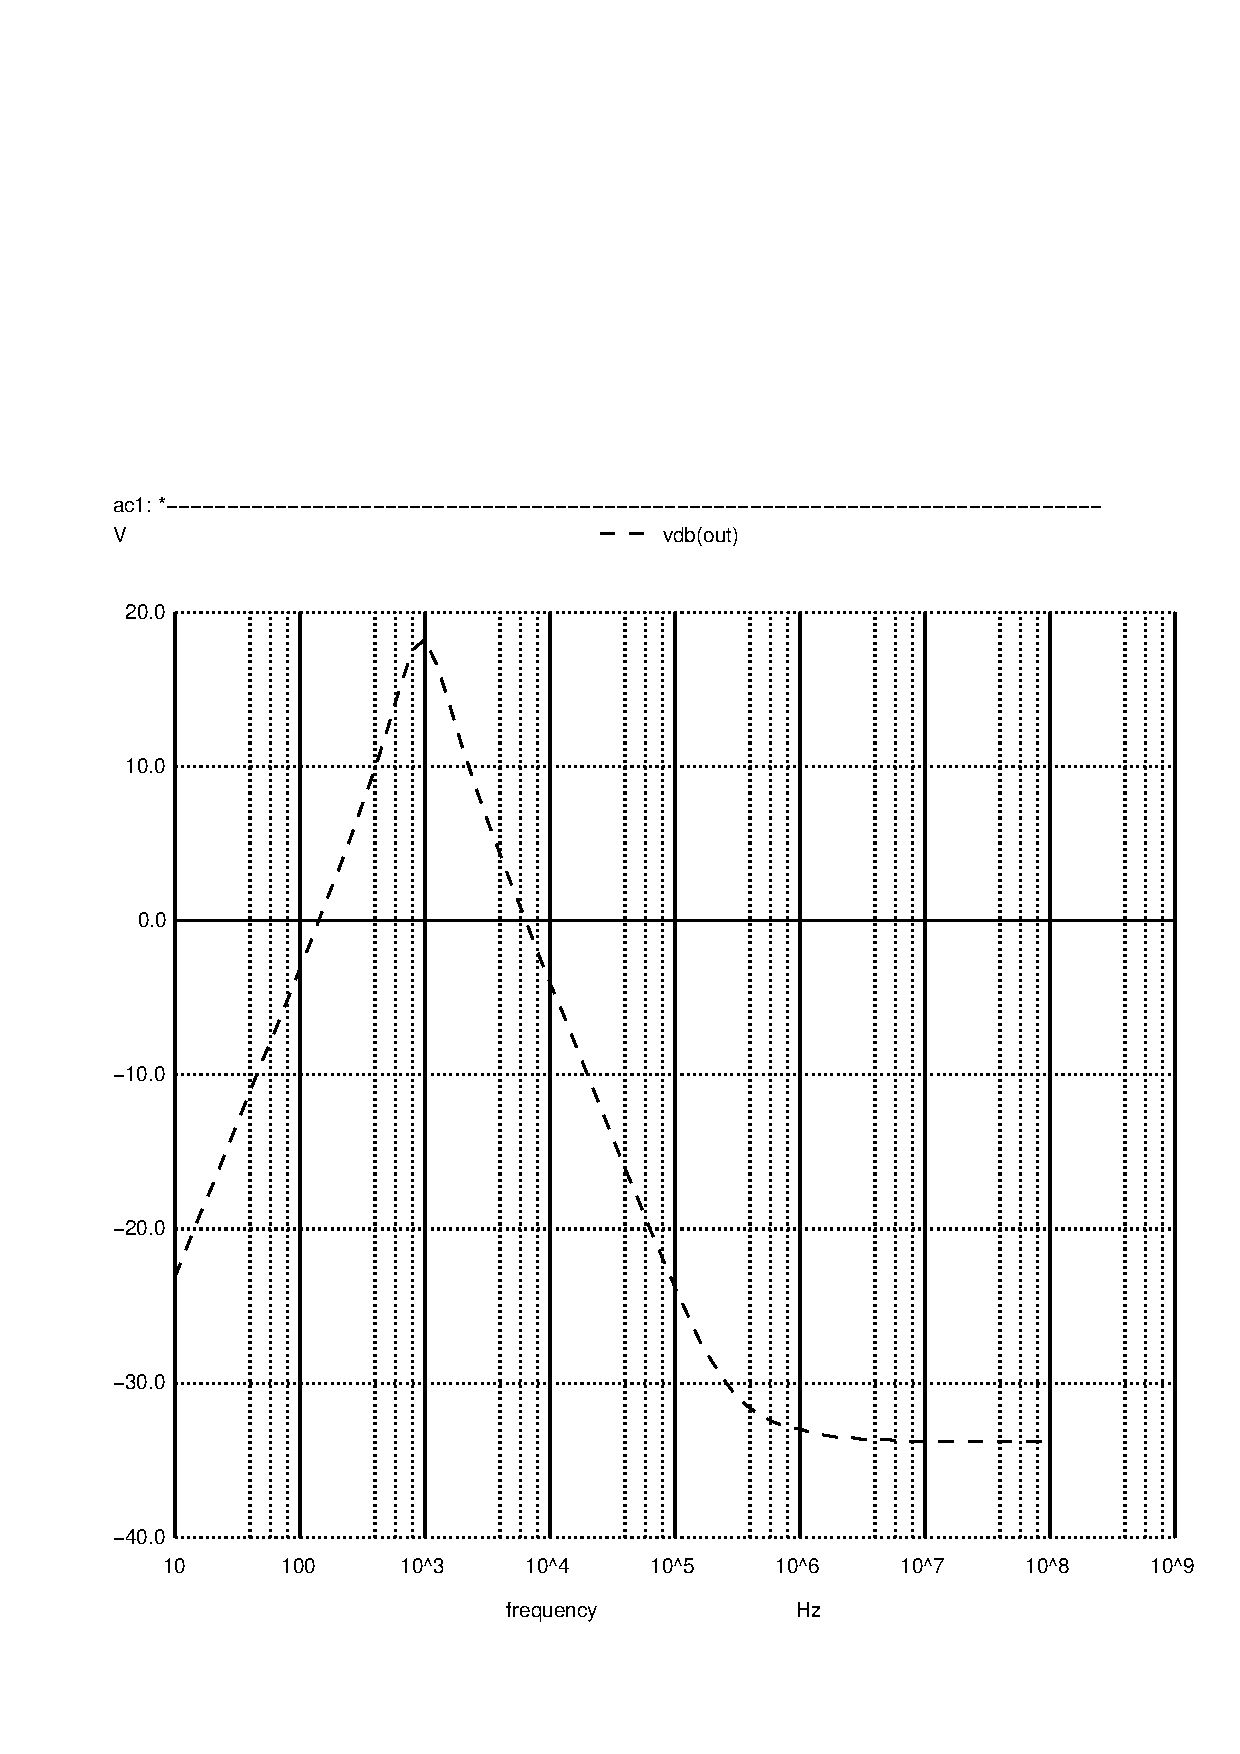
\includegraphics[width=\linewidth, clip]{gain.pdf}
    \end{subfigure}
    \caption{Gain in dB as function of log(f); Left (Octave) and right (Ngspice) }
    \label{fig:argTOct}
\end{figure*}

As we can see, the gain obtained and central frequency is very similar between simulation and theoretical. The only considerable difference is from $f = 10^6$ - way above the central frequency -
where the theoretical model graph keeps going down, whereas the simulation stabilizes in a gain of $\approx -35dB$.   

\begin{figure*}[h]
    \centering
    \begin{subfigure}{0.5\textwidth}
      \includegraphics[width=\linewidth, clip]{phase.eps}
    \end{subfigure}
    \begin{subfigure}{0.4\textwidth}
      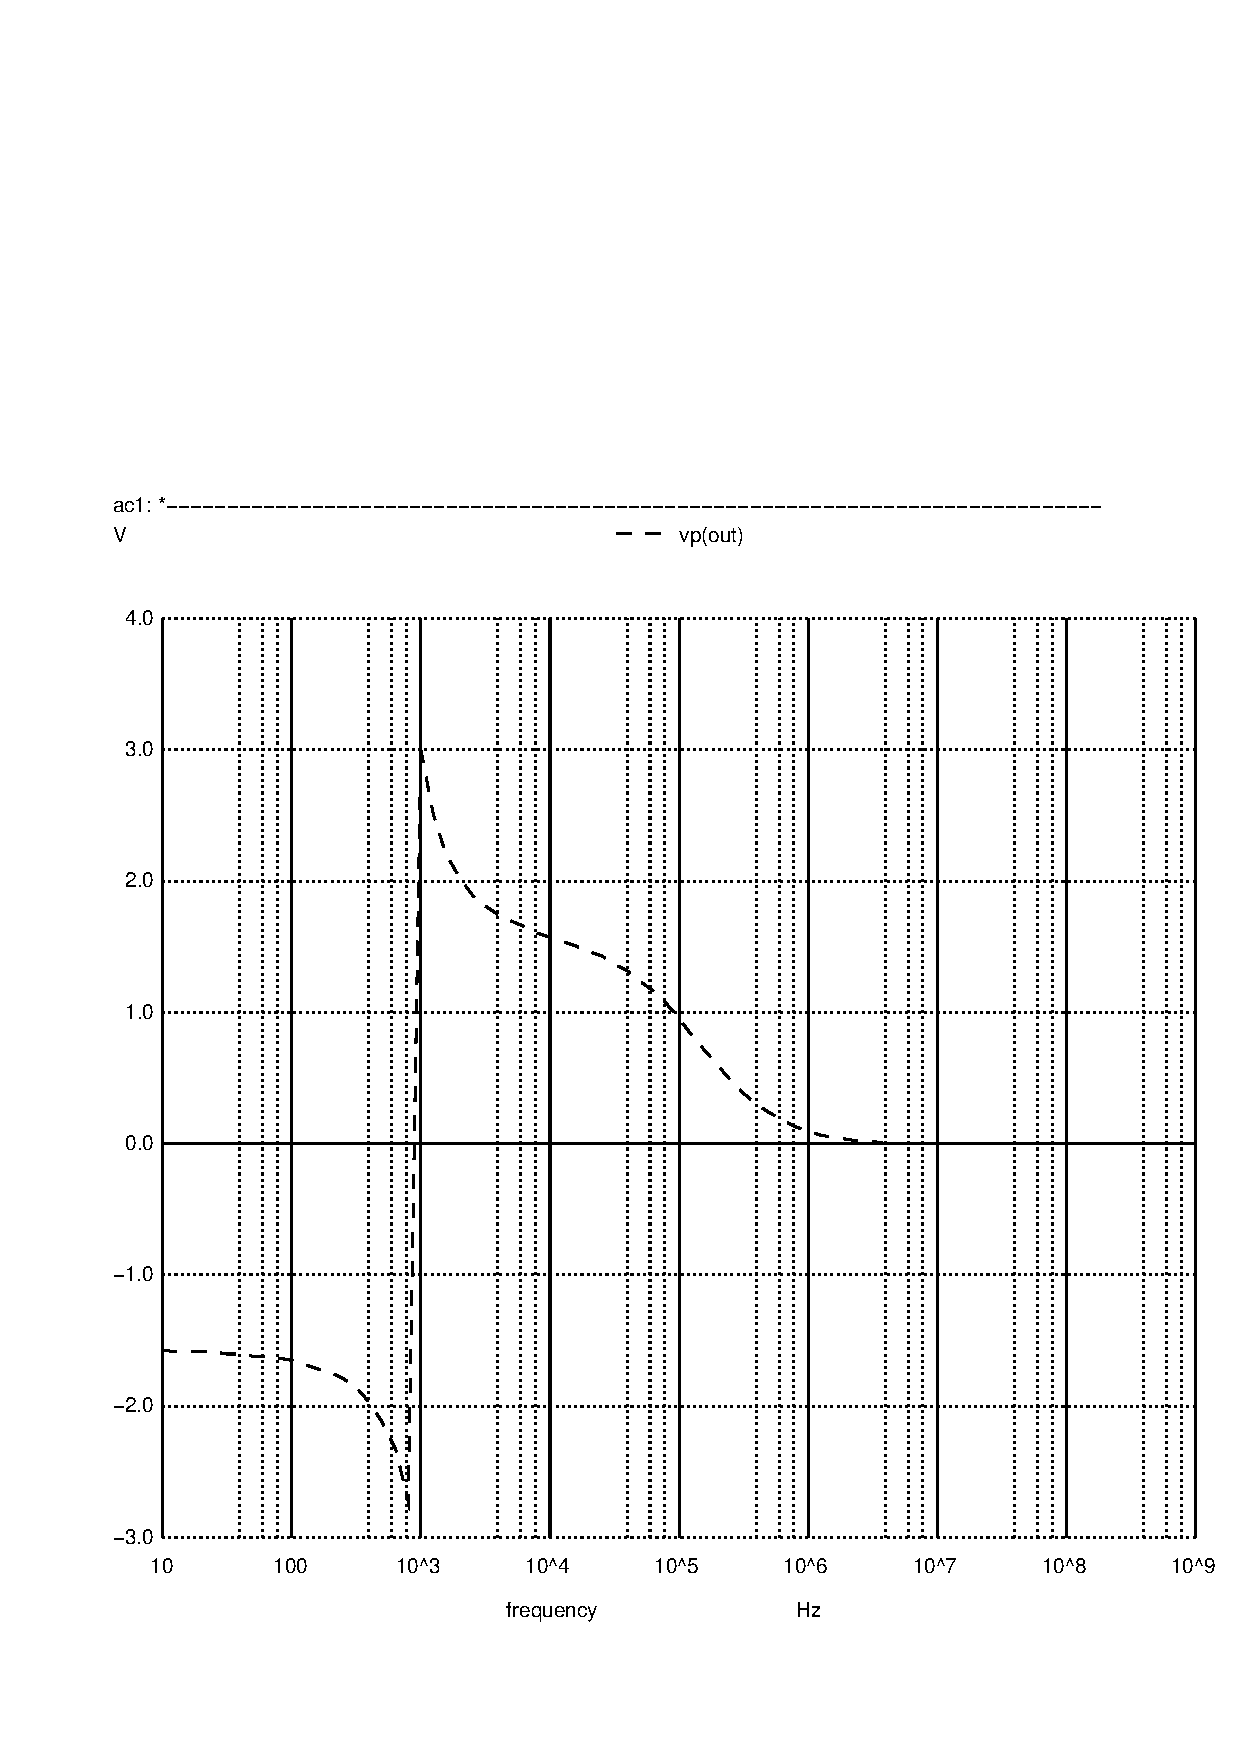
\includegraphics[width=\linewidth, clip]{phase.pdf}
    \end{subfigure}
    \caption{Phase in radians as a function of log(f); Left (Octave) and right (Ngspice) }
    \label{fig:output1}
\end{figure*}

The phase graphs are also very similar until little above the central frequency. Then, the simulated graph goes to 0 whereas the theoretical graph stays asymptotically close to 2.
One possible explanation for this is that the spice model considers two capacitors in the OPAMP model, whereas the ideal model used in the theoritcal analysis does not consider them.

\begin{table}[h]
    % \parbox{.45\linewidth}{
    {
      \centering
      \begin{tabular}{|c|c|c|c|}
        \hline
        $Z_{input}$ & -1.312927e-01\\ \hline
$Z_{output}$ & 0.000000e+00\\ \hline
Max $Gain_{dB}$ & 1.835867e+01\\ \hline
Central frequency [Hz] & 9.660509e+02\\ \hline

      \end{tabular}
      \caption{Side by Side results for impedances, central frequency and gain}
      \label{tab:TheoreticalResults}
    }
\end{table}

Finally, the results shown in the table allow the development of the previous comparison between graphs. As one can see, the central frequency and maximum gain are very similar in both analyses.
On the other hand, the deviation of the impedances is considerable. Firstly, the output impedance is 0 in the ideal model used for the theoretical analysis, so the deviation would always be 100\%.
Secondly, the input impedance difference can be attributed to the same reason observed previously in the graphs: the ideal model of the OPAMP does not take into account the capacitors as
the ngspice model does. 
